\documentclass[12pt]{article}
\usepackage[margin=1in]{geometry}
\usepackage[utf8]{inputenc}
\usepackage{graphicx}
\usepackage{pgfgantt}
\usepackage[table]{xcolor}

% --- CUSTOMIZATION TO KEEP ABSTRACT AT 12PT ---
\renewenvironment{abstract}
 {\begin{center}
  \bfseries \abstractname\vspace{-.5em}\vspace{0pt}
  \end{center}
  \list{}{
    \listparindent 0.5cm
    \itemindent    \listparindent
    \leftmargin    0pt        % Standard text margins
    \rightmargin   \leftmargin
    \parsep        0pt
  }
  \item\relax}
 {\endlist} 
% ----------------------------------------------

\title{\large A DEEP LEARNING-BASED POST-PROCESSOR FOR RESTORING LOW-BITRATE JPEG2000 IMAGES}
\author{
    Jayden Lewis \\ 
    \small \texttt{jilewis@ualberta.ca}
    \and 
    Shubh Jha \\ 
    \small \texttt{sjha3@ualberta.ca}
    \and
    Ritish Pentapalli \\ 
    \small \texttt{pentapal@ualberta.ca} 
}
\date{}

\begin{document}

\maketitle

\begin{abstract}
Previous approaches to image restoration typically focus on removing blocking artifacts from standard JPEG images using Convolutional Neural Networks (CNNs). However, in bandwidth-constrained environments where images are compressed using JPEG2000 at ultra-low bitrates (0.05-0.15 bpp), artifacts are often dominated by a "ringing effect" around sharp edges. Standard restoration techniques, such as gaussian or median filtering, often blur these salient edges in an attempt to remove these ripples, rendering text and fine details illegible. This project proposes a method to reconstruct edges in such ultra-low bitrate JPEG2000 compressed images, using a deep-learning based approach that utilizes a Dual-Domain Loss Function (combining Pixel Loss and Frequency Loss), improving visual perceptibility. We hypothesize that this combination will work better than existing spatial-only techniques by explicitly targeting the high-frequency signature of ringing artifacts while preserving structural details.
\end{abstract}

\section*{{\large I}\small{NTRODUCTION}}

\quad \, Digital image compression is the cornerstone of modern multimedia communication, enabling the efficient transmission of high-resolution visual data. The fundamental principle behind lossy compression is to remove visually imperceptible features in images, typically achieved by transforming image data into the frequency domain and discarding less perceptually significant coefficients. However, this efficiency comes at a cost; the choice of compression standard dictates the nature of the resulting visual degradation. \\

Standard JPEG, a ubiquitous format for digital photography, relies on the Discrete Cosine Transform (DCT), which processes images in independent $8\times8$ pixel blocks [1, 2]. At low bitrates, this independence causes visible discontinuities at block boundaries, known as "blocking artifacts" [1]. \\

Considering its popularity, significant research has been dedicated to artifact reduction in such JPEG images. However, comparatively little research has been done in artifact reduction for images compressed using JPEG's lesser-known successor, JPEG2000, even more so at ultra-low bitrates. The unique artifacts produced by it remain comparatively under-explored. While JPEG2000  eliminates the "grid-like" blocking artifacts common in JPEG images [3, 4], it suffers from an equally destructive phenomenon known as "ringing artifacts" at extremely low bitrates (0.5-0.15 bpp). As high-frequency wavelet coefficients are quantized or discarded to meet extreme bandwidth constraints, the reconstruction of sharp edges result in oscillating ripples that emanate from high-contrast boundaries, a byproduct of the Gibbs phenomenon [5, 6]. \\

Figure 1 contains a sample image encoded at various bitrates using a JPEG2000 encoder [3], demonstrating that at low bitrates, sharp edges become extremely blurry, and "ring" into neighbouring regions. \\

\begin{figure}[h]
    \centering
    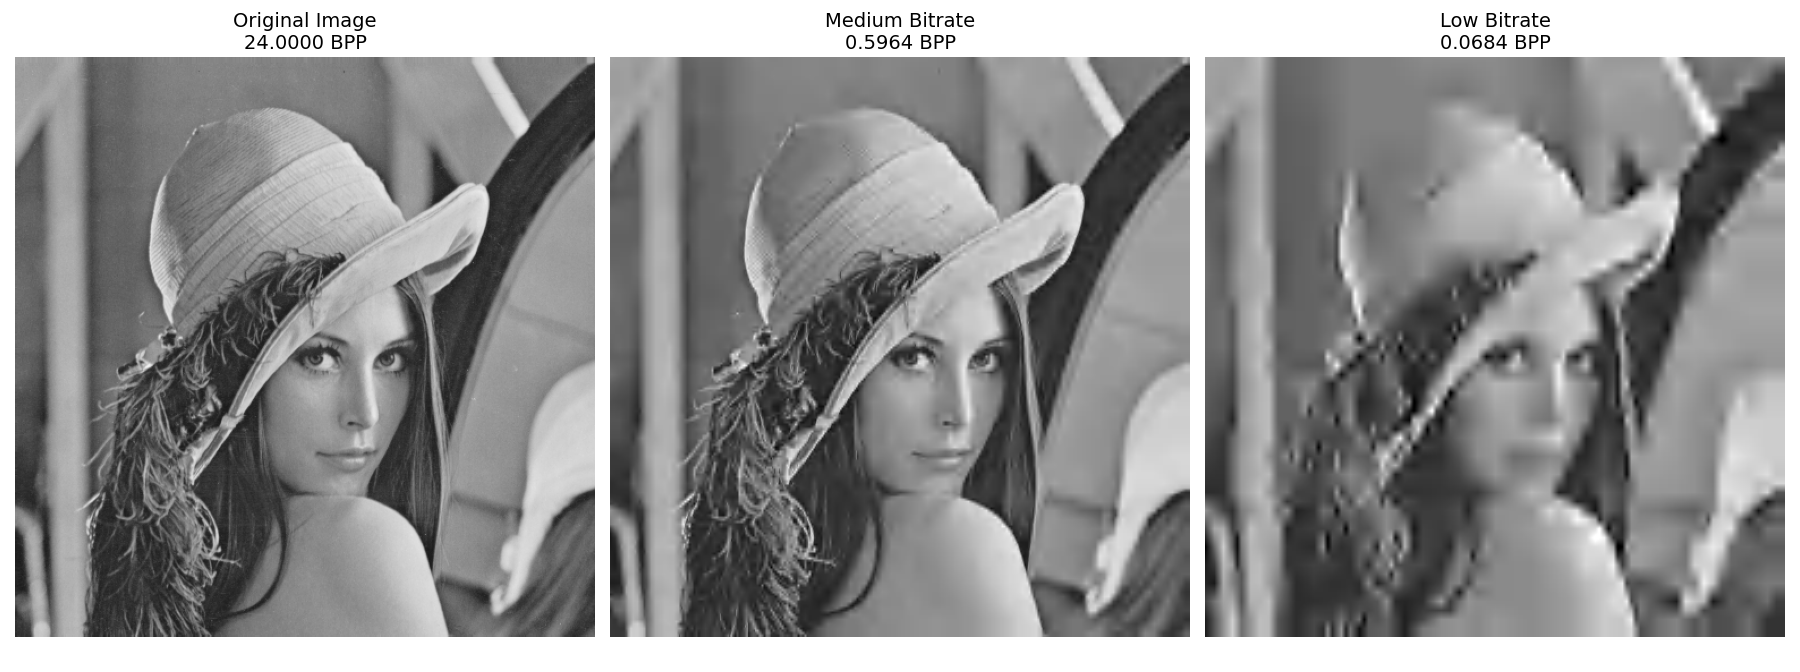
\includegraphics[width=0.8\textwidth]{Figure_1.png}
    \caption{Sample image compressed at various bitrates using JPEG2000}
    \label{fig:timeline}
\end{figure}

In an effort to expand the research sphere targeting this underexplored reconstruction challenge, this project aims to develop a learning-based post-processor specifically for ultra-low bitrate (0.05–0.15 bpp) JPEG2000 images. At these bitrates, ringing artifacts severely degrade the intelligibility of visual data, obscuring fine-grained details such as text and facial features. By moving beyond simple spatial-domain filtering and incorporating frequency-domain awareness, we aim to demonstrate that targeted edge reconstruction is the most effective path toward restoring image quality in bandwidth-constrained environments. \\

To address the challenges mentioned above, this initiative explores a targeted restoration approach designed to mitigate ringing artifacts while preserving edge sharpness. Our methodology is built upon three primary pillars: first, the evaluation of various deep learning architectures to determine which best isolates reconstructs edges; second, the development of a loss function that monitors the image’s "ringing" patterns in the frequency domain using the Fast Fourier Transform (FFT), ensuring the model removes "fake" ripples without blurring details; and third, the curation of a training dataset focused exclusively on distortions found in the ultra-low bitrate setting ($<$ 0.1 bpp). We aim to identify a robust alternative to existing low-bitrate reconstruction methods, providing a pathway toward high-intelligibility multimedia communication in bandwidth-constrained environments. \\

\begin{figure}[h]
    \centering
    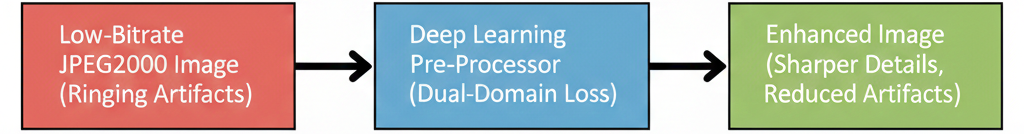
\includegraphics[width=0.8\textwidth]{Figure_2.png}
    \caption{Project at a glance}
    \label{fig:timeline}
\end{figure}

\section*{{\large M}\small{ETHODOLOGY}}

\quad The primary objective of this research is to identify an optimal deep learning configuration for the restoration of ultra-low bitrate JPEG 2000 images. To that extent, the bulk of the work is divded into two primary phases — data synthesis and architecture exploration.

\subsection*{\small{Data Synthesis}}

\quad The construction of a robust training dataset is fundamental to ensuring the model generalizes across a vast array of visual semantics. This research will utilize the LSDIR (Large Scale Dataset for Image Restoration) dataset [7] to provide the necessary scale and diversity. \\

LSDIR comprises over 190,000 high-resolution images, encompassing a comprehensive range of categories including human subjects, complex urban environments, varied natural textures, and man-made objects. This diversity is critical for the project, as the Gibbs phenomenon manifests differently depending on the underlying image content. For instance, ringing artifacts on human facial features require a different restoration sensitivity than those appearing on high-contrast architectural edges. \\

By utilizing a subset of approximately 10,000 diverse images from LSDIR, the risk of the network overfitting to specific high-frequency patterns is significantly mitigated. \\

The degradation pipeline involves compressing these ground-truth images using the OpenJPEG encoder [8] at randomized bitrates within the low regime of 0.5 to 0.15 bpp. This high-volume, multi-semantic approach ensures that the resulting post-processor is capable of restoring quality in real-world scenarios where the subject matter is unpredictable.

\subsection*{\small{Architecture Selection}}

\quad The selection of a neural network architecture is a critical determinant in the efficacy of high-frequency signal recovery. Rather than committing to a single model, a comparative study of several candidate architectures will be conducted to identify the framework best suited for the task. A significant portion of the ongoing literature review is dedicated to analyzing current state-of-the-art [12, 13, 14] in image restoration, in particular, successful implementations in de-blurring and de-noising, to inform the selection of these baseline models. \\

Among the primary candidates for evaluation are Residual Networks (ResNet) [9], which we hypothesize may be particularly effective for this task. By leveraging skip-connections, a ResNet can be trained to isolate the difference between clean ground truth and the corrupted JPEG 2000 input. This approach allows the network to focus on learning the subtractive patterns of the ringing ripples rather than attempting to reconstruct the entire image from first principles. \\

Additionally, hierarchical structures such as the U-Net [10] will be investigated. The encoder-decoder configuration of a U-Net enables the model to capture multi-scale information, where the bottleneck layers identify large-scale oscillating "shadows" while the skip-connections preserve the high-resolution spatial features necessary for sharpening primary edges. \\

Finally, modern Vision Transformers (ViT) [10] will be explored to determine if their global self-attention mechanisms provide a superior receptive field for identifying long-range periodic distortions compared to the local receptive fields of standard convolutional layers. \\

This investigative phase ensures that the final model is not merely a derivative of existing standards but is the result of a rigorous selection process tailored to the specific characteristics of wavelet-based compression artifacts.

\subsection*{\small{Dual-Domain Loss Function}}

\quad The primary technical contribution of this research lies in the development and implementation of a Dual-Domain Loss (DDL) Function. Traditional restoration models are frequently limited by their reliance on spatial-domain metrics (i.e, focusing on pixel-wise loss), which struggle to differentiate between high-frequency structural edges and high-frequency "false" ripples. This research addresses this ambiguity by supervising the network simultaneously in the spatial and spectral domains. \\

The optimization objective is formulated as a weighted combination of two distinct loss components:
$$L_{total} = \alpha L_{spatial} + \beta L_{frequency}$$

\begin{itemize}
    \item Spatial Domain Loss ($L_{spatial}$): This component ensures that the restored image remains anchored to the original pixel intensities. By penalizing absolute differences in the spatial domain, the model preserves the global color accuracy and structural alignment of the scene.
    \item Frequency Domain Loss ($L_{frequency}$): As the core innovation of this project, the frequency loss utilizes the FFT [15] to map image features into the frequency domain. We assume that distinct periodic signatures caused by the Gibbs phenomenon manifest as mathematical artifacts in the frequency domain that are nearly invisible to standard pixel-wise loss functions. By penalizing deviations in the magnitude and phase of the FFT [16, 17], the network is forced to learn the spectral "signature" of a clean edge, effectively teaching the model to distinguish between valid image detail and wavelet-induced noise.
\end{itemize}

The weights, $\alpha$ and $\beta$, will be chosen through experimentation.

\subsection*{\small{Evaluation Metrics}}

\quad Metrics such as Peak Signal-to-Noise Ratio (PSNR) [18] and our proposed DDL provide a baseline for assessing model performance. \\

Structural Similarity Index (SSIM) [19] and Learned Perceptual Image Patch Similarity (LPIPS) [20] may also be evaluated to assess overall performance.

\subsection*{\large{T}\small{IMELINE}}

\quad The project follows a five-week (one for each lab) development cycle. Each week serves as a milestone towards the overall project. \\

\textbf{Lab 1:} This initial phase focuses on curating the 10,000-sample LSDIR subset and establishing the OpenJPEG degradation pipeline. Literature review will begin to identify state-of-the-art architectures suited for restoration. \\

\textbf{Lab 2:} Model development commences with the implementation of baseline architectures, while the literature review concludes to finalize the selection of the primary architecture. Begin training runs on some developed models. \\

\textbf{Lab 3:} Research shifts toward the integration of the project's key innovation: the dual-domain loss function. Comparative testing will continue across selected architectures to evaluate their specific responses to spectral-domain supervision. \\

\textbf{Lab 4:} Intensive model optimization is conducted by tuning the weighting coefficients between spatial and frequency penalties. \\

\textbf{Lab 5:} The final week is dedicated to refining the trained post-processor and generating visual qualitative comparisons. All experimental findings and architectural insights are synthesized into the final research report. \\

\begin{center}
\renewcommand{\arraystretch}{1.8}
\setlength{\tabcolsep}{10pt}
\begin{tabular}{|l|c|c|c|c|c|}
\hline
\textbf{Task} & \textbf{Week 1} & \textbf{Week 2} & \textbf{Week 3} & \textbf{Week 4} & \textbf{Week 5} \\ \hline
Data Synthesis & \cellcolor{red!60} & & & & \\ \hline
Literature Review & \multicolumn{2}{c|}{\cellcolor{orange!60}} & & & \\ \hline
Model Dev. \& Training & & \multicolumn{3}{c|}{\cellcolor{cyan!60}} & \\ \hline
Refinement \& Comparison & & & \multicolumn{2}{c|}{\cellcolor{green!60}} & \\ \hline
Final Report Writing & & & & & \cellcolor{purple!40} \\ \hline
\end{tabular}
\caption{Project timeline at a glance}
\end{center}

\section*{\large{C}\small{ONCLUSION}}

\quad This research proposal outlines a rigorous approach to addressing the fundamental limitations of wavelet-based compression through deep learning-based post-processing. \\

The primary technical contribution of our work includes the idealization of a Dual-Domain Loss function. By supervising the network in both the spatial and frequency domain, the model is equipped to specifically target and suppress the periodic oscillations characteristic of the Gibbs phenomenon without sacrificing edge integrity. The effectiveness of this strategy will be verified through perceptually-aware metrics such as SSIM and LPIPS, ensuring that the final output provides a measurable increase in image intelligibility. \\

Ultimately, this project aims to provide a robust solution for ultra-low bitrate JPEG 2000 restoration, demonstrating that deep learning configurations can effectively bridge the gap between high compression efficiency and visual clarity.


% --- KEEPING REFERENCES AT 12PT ---
\renewcommand{\refname}{\selectfont References} % Prevents size change
\begin{thebibliography}{9}
\itemsep 0pt
\bibitem{jpeg}
G. K. Wallace, “The JPEG still picture compression standard,” IEEE Transactions on Consumer Electronics, 1992.

\bibitem{dct}
N. Ahmed, T. Natarajan, and K. R. Rao, “Discrete cosine transform,” IEEE Transactions on Computers, 1974.

\bibitem{jpeg2000}
D. Taubman and M. Marcellin, \textit{JPEG2000 Image Compression Fundamentals, Standards and Practice}, Springer, 2002.

\bibitem{ebcot}
D. Taubman, “High performance scalable image compression with EBCOT,” IEEE Transactions on Image Processing, 2000.

\bibitem{gibbs}
J. Willard Gibbs, “Fourier’s series,” Nature, 1898.

\bibitem{ringing}
A. Nosratinia, “Enhancement of JPEG-compressed images by re-application of JPEG,” Journal of VLSI Signal Processing, 2001.

\bibitem{lsdir}
J. Li et al., “LSDIR: A Large Scale Dataset for Image Restoration,” arXiv, 2023.

\bibitem{openjpeg}
OpenJPEG Consortium, “OpenJPEG: An open-source JPEG2000 codec,” 2015.

\bibitem{resnet}
K. He et al., “Deep residual learning for image recognition,” CVPR, 2016.

\bibitem{unet}
O. Ronneberger et al., “U-Net: Convolutional networks for biomedical image segmentation,” MICCAI, 2015.

\bibitem{vit}
A. Dosovitskiy et al., “An image is worth 16x16 words: Transformers for image recognition at scale,” ICLR, 2021.

\bibitem{dncnn}
K. Zhang et al., “Beyond a Gaussian denoiser: Residual learning of deep CNN for image denoising,” IEEE TIP, 2017.

\bibitem{edsr}
B. Lim et al., “Enhanced deep residual networks for single image super-resolution,” CVPR Workshops, 2017.

\bibitem{restormer}
S. Zamir et al., “Restormer: Efficient transformer for high-resolution image restoration,” CVPR, 2022.

\bibitem{fft}
J. W. Cooley and J. Tukey, “An algorithm for the machine calculation of complex Fourier series,” Mathematics of Computation, 1965.

\bibitem{frequencyloss}
Y. Jiang et al., “Focal frequency loss for image reconstruction and synthesis,” ICCV, 2021.

\bibitem{fourierloss}
L. Yang and Z. Sun, “Image restoration using Fourier domain losses,” IEEE Access, 2020.

\bibitem{psnr}
Z. Wang and A. Bovik, “Mean squared error: Love it or leave it?” IEEE Signal Processing Magazine, 2009.

\bibitem{ssim}
Z. Wang et al., “Image quality assessment: From error visibility to structural similarity,” IEEE TIP, 2004.

\bibitem{lpips}
R. Zhang et al., “The unreasonable effectiveness of deep features as a perceptual metric,” CVPR, 2018.

\end{thebibliography}

\clearpage

\begin{center}
  \section*{{\large L}\small{ITERATURE} {\large R}\small{EVIEW}} 
\end{center}

\vspace{20}

\subsection*{Introduction}

\quad \, The restoration of compressed images has historically relied on classical signal processing techniques that operate primarily in the spatial domain. For wavelet-based compression standards like JPEG2000, the primary restoration challenge is the Gibbs phenomenon, which occurs when high-frequency coefficients are discarded to meet extreme bandwidth constraints—typically between 0.05 and 0.15 bpp [1]. This results in "ringing" artifacts, characterized by oscillating ripples that around high-contrast edges [1]. Early attempts to mitigate these ripples often utilized linear smoothing filters, such as Gaussian or median filters, which operate on the assumption that artifacts are high-frequency noise [2]. However, these methods frequently fail to distinguish between the periodic "fake" ripples of the ringing effect and the actual high-frequency structural details of the image [2]. \\

The fundamental limitation of these classical approaches lies in a rigid trade-off between artifact suppression and edge preservation. Since ringing artifacts are mathematically tied to the reconstruction of sharp boundaries, aggressive spatial filtering intended to remove ripples inherently blurs salient edges, rendering fine details and text illegible. This "smoothing problem" is exacerbated in ultra-low bitrate environments where the signal-to-artifact ratio is exceptionally low. While transform-domain methods and iterative restoration techniques like Projection onto Convex Sets (POCS) attempted to introduce edge-awareness, they often lacked the sophistication to model the complex, non-linear distortions produced by modern wavelet-based encoders [3]. This persistent gap in restoration quality necessitated a shift toward more adaptive, data-driven frameworks. \\

The limitations of classical filtering and transform-based post-processing methods motivated a paradigm shift toward data-driven restoration models. With the emergence of Convolutional Neural Networks (CNNs), artifact removal began to be formulated as a supervised learning problem, where a network is trained to directly map compressed images to their uncompressed counterparts. \\

Dong et al. made a seminal contribution in this direction by proposing the Artifact Reduction Convolutional Neural Network (AR-CNN) [4]. AR-CNN is a four-layer fully convolutional architecture that treats compression artifact removal as an end-to-end regression problem. It suppresses multiple artifact types simultaneously, including blocking, ringing, and blurring effects. \\

Despite these advances, AR-CNN is trained solely on an image’s spatial-domain, i.e., pixels, with the goal of optimising the mean squared error (MSE) loss between reconstructed and ground-truth pixels. While this approach reduces visible discontinuities, it frequently results in overly smoothed reconstructed images and limited recovery of high-frequency details at high compression rates.
Subsequent CNN-based approaches delve deeper into residual architectures [5, 6]. However, like AR-CNN, they treat artifact removal as a spatial regression problem, demonstrating that CNNs outperform hand-crafted filters while relying heavily on pixel-domain losses. \\

\subsection*{Limitations of Spatial-Loss Based Approaches}

\quad \, Two major limitations emerge from these spatial CNN frameworks:

\begin{itemize}
    \item \textbf{Frequency Blindness:} Spatial MSE-trained CNNs do not enforce consistency in the frequency domain. The AR-CNN experiments [4] show that ringing artifacts originate from the coarse quantization of high-frequency Discrete Cosine Transform (DCT) components, a manifestation of the Gibbs phenomenon. However, because the training objective does not directly penalize spectral inconsistencies, the model often understates the restoration of fine structural details [7].
    
    \item \textbf{Low Bitrate Instability:} As compression quality decreases, the complexity and intensity of artifacts increase. While AR-CNN is capable of raising the Peak Signal-to-Noise Ratio (PSNR), the restored outputs frequently exhibit residual ringing. This suggests that purely spatial supervision struggles to resolve the complex distortions introduced by high levels of quantization [8].
\end{itemize}

These observations indicate that although CNNs offer a robust framework for learning compression priors, spatial-domain architectures by themselves may not entirely capture frequency-specific distortions induced by transform-based compression [9]. Their reliance on pixel-level loss functions and the lack of explicit spectral supervision highlights a significant gap, particularly when working with frequency distortion and low-bitrate compression scenarios [9].

\subsection*{Wavelet-Based Methods and Deep Learning}


\quad \, To address the historical limitations of hand-crafted thresholds, recent research has moved toward integrating wavelet theory with deep learning architectures. A primary development in this area is the Wavelet-like Auto-Encoder (WAE) introduced by Liu et al. [13]. Instead of relying on a standard Discrete Wavelet Transform (DWT), the WAE utilizes a learnable encoding layer that decomposes an input image into low-resolution low-frequency ``profile'' channels and high-frequency ``detail'' channels. This hybrid approach offers several advantages: the network can learn to preserve discriminative content in the profile channel while isolating the oscillations characteristic of ringing artifacts in the detail channels [14]. Furthermore, by utilizing a reconstruction constraint during training, the auto-encoder ensures that the decomposed channels retain enough information to synthesize the original image accurately while maintaining high performance with lower computational complexity [15]. \\

Building upon the WAE concept, recent frameworks such as the Frequency and Spatial Interactive (FSI) network have sought to combat ``spectral bias,'' which is the tendency of neural networks to favor low-frequency global structures over high-frequency details [16]. These modern architectures often utilize parallel branches, where a dedicated frequency learning block employs Fourier transforms to directly identify and eliminate redundant spectral signatures in the frequency domain [17]. This is frequently paired with a concurrent spatial branch that restores local textures using hierarchical structures. By facilitating constant feature exchange between these domains through interactive fusion, the model prevents the oversmoothing typical of spatial-only CNNs and ensures that edge restoration is guided by spectral consistency [18]. \\

Further advancements include the development of Multi-branch Dynamic Selective Frequency Networks (SFNet), which introduce a content-aware approach to restoration [19]. Unlike traditional wavelet auto-encoders that use fixed sub-band decompositions, these networks utilize dynamic modules to separate feature maps into different frequency components based on the specific degradation of the input. By employing channel-wise attention mechanisms, the network can accentuate the most informative components required for reconstruction [20]. This is particularly effective for ultra-low bitrate JPEG2000 artifacts, as it allows the model to ignore ``fake'' ripples while emphasizing true structural edges. Complementing these architectural changes is the implementation of Focal Frequency Loss (FFL), which provides a differentiable distance metric in the frequency domain [21]. This loss function allows a model to adaptively focus on hard-to-synthesize frequencies by penalizing deviations in both magnitude and phase, ensuring that the final output provides a measurable increase in image intelligibility. \\

\subsection*{Frequency and Spatial-Based Supervision}

\quad \, The fundamental technical contribution of this research lies in the development and implementation of what we have termed as ``Dual-Domain Loss" (DDL) function. So far, it has been highlighted that traditional restoration models are frequently limited by their reliance on spatial-domain metrics, and struggle to differentiate between high-frequency structural edges and ripples [22]. This project addresses this ambiguity by supervising the network simultaneously in the spatial and spectral domains. The optimization objective is formulated as a weighted combination of two distinct loss components: 

$$    L_{total}  = \alpha L_{spatial} + \beta L_{frequency} $$


\quad \, A key idea behind frequency-domain supervision is that different spectral bands are linked to different types of perceptual degradation. Jiang et al. presented Focal Frequency Loss (FFL) and illustrated that the elimination of high-frequency components results in blurring and characteristic ringing artifacts, while the removal of low-frequency components maintains edge contours but modifies global appearance [21]. Their analysis shows that artifacts are not evenly spread out across the spectrum. Instead, distortions show up as localized inconsistencies in certain frequency ranges. This redefines ringing as a structured spectral imbalance rather than a deviation at a pixel level [23]. From this perspective, overseeing restoration in the frequency domain offers a systematic approach to penalize the specific frequency bands accountable for oscillatory artifacts and loss of detail. \\

Notably, Jiang et al. does not propose substituting spatial losses with frequency loss. Instead, they suggest that frequency losses should be included because of the ``spectral bias'' of neural networks, that is, the tendency to learn low-frequency components first while aggressively underfitting high-frequency details [21]. They also highlight a limitation of pixel-wise losses, where every pixel contributes to the objective similarly, making it harder to emphasize under-reconstructed spectral regions [24]. Due to this, networks may reduce global error while still leaving significant frequency gaps. To counter this, they establish a differentiable frequency-domain distance equation derived from the 2D Discrete Fourier Transform (DFT), enabling optimization through stochastic gradient descent [21]. \\

In the frequency domain, each image is shown as a set of complex coefficients $F(u,v)$ that can be broken into amplitude, which represents the energy contribution of each frequency component, and phase, which encodes the spatial alignment and structural position [25]. They demonstrated that minimizing only amplitude differences leads to strange color patterns, while minimizing only phase leads to noise-like reconstructions. However, the reconstruction matches the ground truth only when both are taken into account. FFL solves this problem by weighting hard spectral components adaptively, which makes the network pay more attention to frequency ranges that remain mismatched [26]. \\


Recent advancements have moved beyond simple loss functions toward architectures that perform real-time, bidirectional cross-domain feature fusion [27]. The Frequency-Aware Network (FreANet) and CDFFNet demonstrate that explicitly modeling frequency-domain characteristics effectively mitigates interference and enhances detail preservation [28]. These models utilize a Multi-Domain Feature Extractor (MDFE) to adaptively aggregate spatial and frequency contexts. By facilitating constant feature exchange between these domains, modern frameworks prevent the ``oversmoothing'' typical of spatial-only CNNs [29]. \\


When using wavelet-based compression like JPEG2000, learning in the frequency domain becomes even more important. The Frequency-Aware Guidance framework contends that enforcing consistency exclusively in the spatial domain can distort intricate structural details and advocates for a wavelet-based guidance loss functioning concurrently in both spatial and frequency representations [30]. The success of these existing dual-domain methods serves to demonstrate that our aim to utilize frequency as well as spectral supervision is in the right direction. By leveraging these insights, it becomes clear that because ringing artifacts are stronger near edges (areas with high-frequency wavelet coefficients), frequency-aware supervision is a robust method to keep edges sharp while eliminating oscillatory distortions. This aligns with our project goal of targeting ultra-low bitrate JPEG2000 ringing while preserving structural detail.

\subsection*{Evaluation Metrics and the Perception-Distortion Tradeoff}

\quad \, A critical challenge in restoring images at ultra-low bitrates is determining what constitutes a ``successful" restoration. Traditionally, image restoration has relied on signal-fidelity metrics such as PSNR, but recent theoretical and empirical studies have demonstrated that these metrics often fail to capture the visual nuances required for human perception. This section explores the fundamental tradeoff between signal accuracy and perceptual realism and establishes the multi-metric benchmarking standard used in modern research. \\

Blau and Michaeli's work suggests that distortion metrics (such as PSNR and SSIM) and perceptual quality (the degree to which an image looks "natural") are often mutually exclusive [32]. Standard models aiming to minimize Mean Squared Error (MSE) often produce blurry, unnatural reconstructions because the model seeks an "average" solution among possible ground-truth candidates. They showed that there is a mathematically unattainable region in the perception-distortion plane; an algorithm cannot maximize signal accuracy while simultaneously achieving perfect perceptual realism. \\

To navigate this tradeoff, modern restoration research employs a three-pronged evaluation strategy to ensure a holistic assessment of the model.

\begin{itemize}
    \item \textbf{PSNR}: Peak Signal-to-Noise Ratio is retained to measure objective signal fidelity and pixel-level accuracy. While it is the standard for measuring noise suppression, it often correlates poorly with perceived sharpness.
    \item \textbf{SSIM}: The Structural Similarity Index evaluates image quality based on the degradation of structural information, specifically luminance, contrast, and patterns [34]. While SSIM correlates better with subjective quality than MSE, it can still struggle to distinguish between genuine edges and the periodic oscillations of ringing artifacts.
    \item \textbf{LPIPS}: Learned Perceptual Image Patch Similarity utilizes the internal activations of deep networks (such as VGG-16) to measure ``perceptual distance" [35]. This metric has been found to correspond to human judgments far more accurately than SSIM or PSNR, particularly in cases involving geometric distortions or fine textures.
\end{itemize}

\quad \, This benchmarking approach allows for the identification of ``admissible" models that strike a more optimal balance between mathematical precision and visual clarity.

\subsection*{Conclusion}

\quad \, The landscape of image restoration is currently undergoing a paradigm shift, moving from simple spatial filters toward complex, multi-domain frameworks that recognize images as both spatial structures and spectral signals. \\

Our proposed research seeks to contribute to this growing sphere by explicitly bridging the gap between classical wavelet theory and modern deep learning. By focusing on the unique challenges of ultra-low bitrate JPEG2000 compression, we aim to extend the existing research on dual domain reconstruction. Ultimately, this project serves not only to improve the intelligibility of bandwidth-constrained visual data but also to refine our understanding of how frequency-aware architectures can better mimic the structural and spectral sensitivity of human perception.


\renewcommand{\refname}{\selectfont References (Literature Review)} % Prevents size change
\begin{thebibliography}{9}

\bibitem{nosratinia2003}
A. Nosratinia, "Post-processing of JPEG-2000 images to remove compression artifacts", IEEE Signal Processing Letters, vol. 10, no. 10, pp. 296-299, 2003.

\bibitem{gonzalez2018}
R. C. Gonzalez and R. E. Woods, Digital Image Processing, 4th ed. Pearson, 2018.

\bibitem{berkner2001}
K. Berkner and E. L. Schwartz, "Smoothness-constrained projection onto convex sets for reduction of tiling artifacts in JPEG 2000", Applications of Digital Image Processing XXIV, SPIE, 2001.

\bibitem{dong2015}
C. Dong, Y. Deng, C. C. Loy, and X. Tang, "Compression artifacts reduction by a deep convolutional network", in Proc. IEEE Int. Conf. Comput. Vis. (ICCV), Dec. 2015, pp. 576–584.

\bibitem{zhang2017}
K. Zhang, W. Zuo, Y. Chen, D. Meng, and L. Zhang, "Beyond a Gaussian denoiser: Residual learning of deep CNN for image denoising", IEEE Transactions on Image Processing, vol. 26, no. 7, pp. 3142-3155, 2017.

\bibitem{lim2017}
B. Lim, S. Son, H. Kim, S. Nah, and K. M. Lee, "Enhanced deep residual networks for single image super-resolution", Proceedings of the IEEE Conference on Computer Vision and Pattern Recognition (CVPR) Workshops, 2017, pp. 136-144.

\bibitem{jiang2021}
L. Jiang, B. Dai, W. Wu, and C. C. Loy, "Focal Frequency Loss for Image Reconstruction and Synthesis", in Proceedings of the IEEE/CVF International Conference on Computer Vision (ICCV), 2021, pp. 13919-13929.

\bibitem{xu2020}
K. Xu, M. Ye, G. Zhang, J. Wu, Z. Hou, and W. Yin, "Learning in the Frequency Domain", in Proceedings of the IEEE/CVF Conference on Computer Vision and Pattern Recognition (CVPR), 2020, pp. 1740-1749.

\bibitem{xiao2022}
J. Xiao et al., "Frequency-Aware Guidance for Image Restoration", IEEE Transactions on Image Processing, vol. 31, pp. 4642-4657, 2022.

\bibitem{zamir2020}
S. W. Zamir et al., "Learning Enriched Features for Real-Image Restoration and Enhancement," in Proc. Eur. Conf. Comput. Vis. (ECCV), 2020.

\bibitem{zhang2023_fourier}
H. Zhang et al., "Deep Fourier-Based Exposure Correction Network with Spatial-Frequency Interaction," IEEE Trans. Image Process., vol. 32, 2023.

\bibitem{gu2021}
J. Gu et al., "Interpretable Image Restoration with Frequency Domain Constraints," in Proc. IEEE/CVF Conf. Comput. Vis. Pattern Recognit. (CVPR), 2021.

\bibitem{liu2021_wae}
T. Liu et al., "Wavelet-based Network for Image Restoration," IEEE Access, vol. 9, 2021.

\bibitem{liu2018_mwcnn}
P. Liu et al., "Multi-level Wavelet Convolutional Neural Networks," IEEE Access, vol. 6, 2018.

\bibitem{zhang2019_wavelet}
J. Zhang et al., "Wavelet Integrated CNNs for Noise-Robust Image Classification," in Proc. IEEE/CVF Conf. Comput. Vis. Pattern Recognit. (CVPR), 2019.

\bibitem{wang2022_fsi}
Z. Wang et al., "Spatial-Frequency Interaction Network for Real-World Image Super-Resolution," in Proc. IEEE/CVF Conf. Comput. Vis. Pattern Recognit. (CVPR), 2022.

\bibitem{rao2021_gfnet}
Y. Rao et al., "Global Filter Networks for Image Classification," in Adv. Neural Inf. Process. Syst. (NeurIPS), 2021.

\bibitem{li2023_mutual}
C. Li et al., "Spatial-Frequency Mutual Learning for Image Restoration," in Proc. AAAI Conf. Artif. Intell., 2023.

\bibitem{fang2023_sfnet}
M. Fang et al., "Selective Frequency Network for Image Restoration," arXiv preprint arXiv:2303.04100, 2023.

\bibitem{hu2018_senet}
J. Hu et al., "Squeeze-and-Excitation Networks," in Proc. IEEE Conf. Comput. Vis. Pattern Recognit. (CVPR), 2018.

\bibitem{ledig2017}
C. Ledig et al., "Photo-Realistic Single Image Super-Resolution Using a Generative Adversarial Network," in Proc. IEEE Conf. Comput. Vis. Pattern Recognit. (CVPR), 2017.

\bibitem{yu2021_dual}
X. Yu et al., "Dual-Domain Deep Convolutional Network for Compressed Image Restoration," IEEE Trans. Circuits Syst. Video Technol., vol. 31, no. 8, 2021.

\bibitem{zhao2017_loss}
H. Zhao et al., "Loss Functions for Image Restoration with Neural Networks," IEEE Trans. Comput. Imaging, vol. 3, no. 1, 2017.

\bibitem{yang2023_phase}
L. Yang et al., "Phase-Aware Image Restoration Network," in Proc. IEEE/CVF Conf. Comput. Vis. Pattern Recognit. (CVPR), 2023.

\bibitem{chi2020_ffc}
G. Chi et al., "Fast Fourier Convolution," in Adv. Neural Inf. Process. Syst. (NeurIPS), 2020.

\bibitem{xiao2024_cross}
J. Xiao et al., "Cross-Domain Interaction for Image Restoration," IEEE Trans. Image Process., vol. 33, 2024.

\bibitem{chen2024_freq}
Z. Chen et al., "Frequency-Aware Feature Fusion for Compressed Image Enhancement," in Proc. IEEE/CVF Conf. Comput. Vis. Pattern Recognit. (CVPR), 2024.

\bibitem{anwar2020_dense}
S. Anwar et al., "Densely Residual Laplacian Super-Resolution," IEEE Trans. Pattern Anal. Mach. Intell., vol. 42, no. 5, 2020.

\bibitem{yang2022_wavelet_guidance}
W. Yang et al., "Wavelet-based Guidance for Deep Image Restoration," IEEE Trans. Image Process., vol. 31, 2022.

\bibitem{lai2018_lapsrn}
W. S. Lai et al., "Fast and Accurate Image Super-Resolution with Deep Laplacian Pyramid Networks," IEEE Trans. Pattern Anal. Mach. Intell., vol. 41, no. 11, 2018.

\bibitem{fu2021_edge}
X. Fu et al., "Edge-aware Deep Image Restoration," IEEE Trans. Image Process., vol. 30, 2021.

\bibitem{blau2018_tradeoff}
Y. Blau and T. Michaeli, "The Perception-Distortion Tradeoff," in Proc. IEEE Conf. Comput. Vis. Pattern Recognit. (CVPR), 2018.

\bibitem{wang2004_ssim}
Z. Wang et al., "Image Quality Assessment: From Error Visibility to Structural Similarity," IEEE Trans. Image Process., vol. 13, no. 4, 2004.

\bibitem{zhang2018_lpips}
R. Zhang et al., "The Unreasonable Effectiveness of Deep Features as a Perceptual Metric," in Proc. IEEE Conf. Comput. Vis. Pattern Recognit. (CVPR), 2018.

\bibitem{agustsson2017_div2k}
E. Agustsson and R. Timofte, "NTIRE 2017 Challenge on Single Image Super-Resolution: Dataset and Study," in Proc. IEEE Conf. Comput. Vis. Pattern Recognit. (CVPR) Workshops, 2017.

\bibitem{li2023_lsdir}
Y. Li et al., "LSDIR: A Large Scale Dataset for Image Restoration," arXiv preprint arXiv:2308.02523, 2023.

\end{thebibliography}

\end{document}